\chapter[Hydrostatic Primitive Equations]{Hydrostatic Primitive Equations}
\label{chapter:4}

To begin working on 3D simulations of the ocean, we began with the most commonly used set of governing equations: the hydrostatic primitive equations \cite{96Mcw}.  

\section{Physical Model and Governing Equations}

The hydrostatic primitive equations are the Navier-Stokes equations with under the effect or rotation and assuming hydrostatic pressure (details in Section \ref{derivegoverningeqns}).  In addition, there is conservation of mass (incompressible) and an open lid condition governed by a kinematic boundary condition.  
%
\begin{equation*}\label{e:seasurfaceheight}
\frac{\partial \eta}{\partial t} + ({\bf u_h} |_{\rm z=z_{max}}) \cdot \nabla_{\rm h} \eta  =  (w|_{\rm z=z_{max}})
\end{equation*}

\begin{equation*} \label{e:momentum}
\frac{\partial {\bf u}_{h}}{\partial t} + {\bf u} \cdot \nabla {\bf u}_{h} + \frac{1}{Ro} f \hat{\bf k} \times {\bf u}_{h}= -\nabla_{h} P + \frac{1}{Re} \nabla ^{2} {\bf u}_{h}
\end{equation*}

\begin{equation*}\label{e:continuity}
 \frac{\partial w}{\partial z} = - \nabla_{\rm h}{\bf u_h}, (w|_{\rm z=z_{bottom}({\bf x_{h}})})
\end{equation*}

\begin{equation*}\label{e:hydrostaticpressure}
\frac{\partial P}{\partial z} = -\frac{1}{Fr^{2}}, P|_{z=z_{max}} = \frac{\eta}{Fr^{2}}
\end{equation*}
%
Currently, a constant eddy viscosity model is being used for turbulence modeling.  Also, for development purposes, there is no stratification and no tracking of the scalar transport variables.  After all the features and numerics are fully implemented and tested, more sophisticated turbulence modeling and variable density capabilities will be added.  Additionally, the Coriolis effect is not incorporated in any of the 2D results.

To start, an analytic linearized solution was used for initialization (no forcing and periodic boundaries).  The numerical results converged to the analytic linearized solution within the numerical accuracy of the method.  This case has been used for testing convergence of any numerical techniques added or developed specifically for ocean modeling capabilities.

For most of the work presented here, the test case used is a 2D wind-driven model that is initially at rest.  The wind is incorporated through the forcing term in the momentum equation, $\vec{F}_{wind}$.  An analytic function that varies sinusoidally in one horizontal direction and as a gaussian in the vertical direction is used to model the effects of the wind.

\section{Extension of Brinkman Penalization}

The ocean bathymetry is a hugely varying, intricate, and complex surface.  Using current techniques for representation of this bottom boundary results in a surface that is either too crude (stair step representation) or too expensive (body-fitted meshes).  The Brinkman penalization approach combined with an adaptive grid, can make the implementation of complex geometry boundaries accurate and feasible for even a simulation run on a standard desktop computer.

Brinkman penalization works by penalizing the equations in such a way that the boundary conditions are automatically satisfied. This is done by solving the regular governing equations in the fluid region, which is determined by some mask function.  The rest of the computational domain is marked as the solid region and in this region the penalized form of the equations are solved.  Figure \ref{f:diagram} shows a comparison of the stair-step representation of boundary conditions, the Brinkman penalization method and our current implementation (which separates the continental topology and bottom bathymetry).

\begin{center}
\begin{figure}[htp]
\centering
  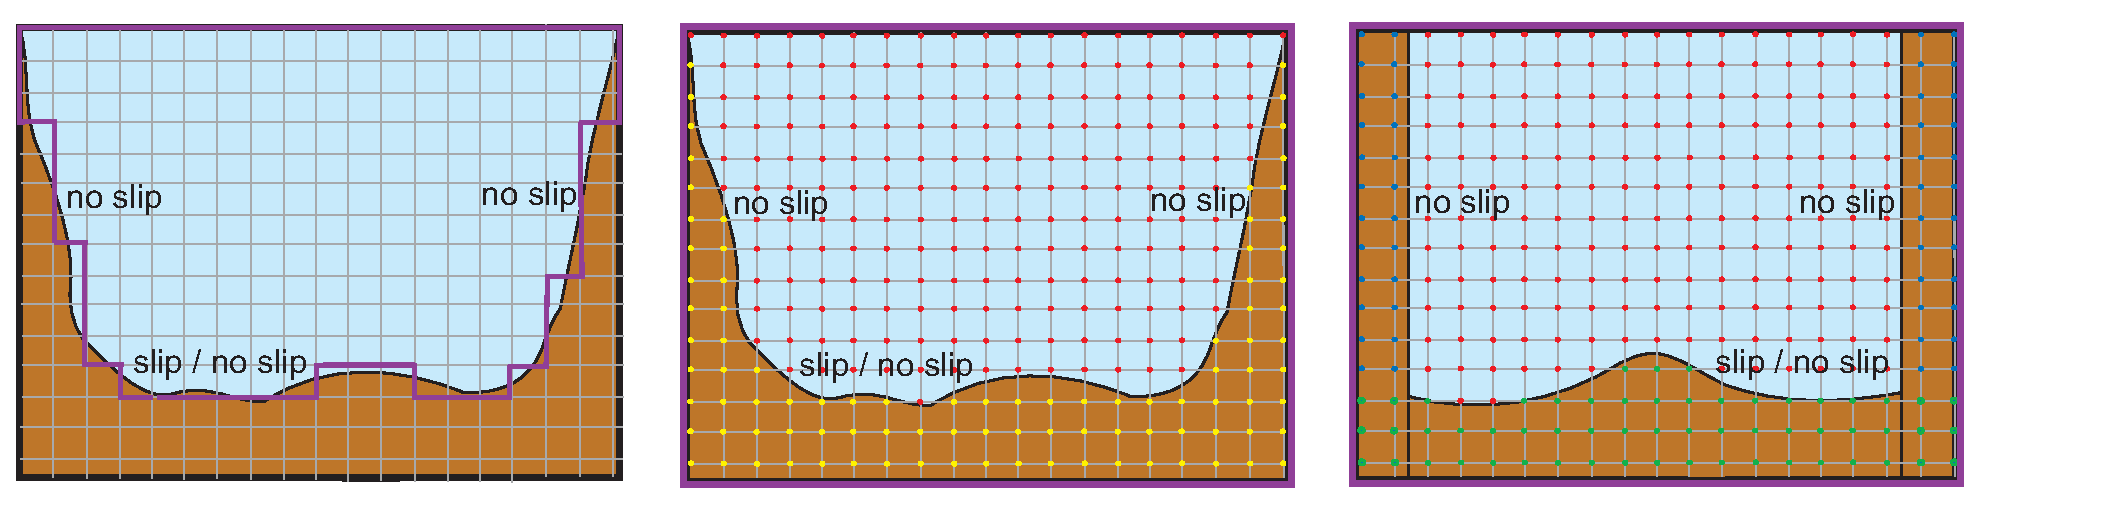
\includegraphics[width=6 in]{Images/diagram_all.eps}
  \caption[Schematic of Brinkman Penalization]{Outlined in purple is computational domain.  Fluid domain is blue and solid domain is brown.  Left: The current stair-step representation of boundary conditions in most ocean models.  Middle: Brinkman Penalization  Right: The current implementation with separation of the continental topology and bottom bathymetry.}\label{f:diagram}
\end{figure}
\end{center}

The incompressible formulation of Brinkman penalization \cite{84AC} is implemented by adding the term, $- \frac{\chi}{\eta_{pen}} {\bf u}$, to the momentum equations.  This term forces the velocity to zero in the Brinkman zone.  As a first attempt to utilize volume penalization to represent ocean boundaries, Brinkman penalization for no slip boundary conditions was used as a benchmark case.  Results are shown in Figure \ref{f:noslip} compared against no slip conditions directly applied to the boundaries.

\begin{center}
\begin{figure}[htp]
\centering
  \includegraphics[width=6 in]{Images/pe_bp_noslip.eps}
  \caption[No slip conditions with and without Brinkman]{Demonstration of no slip boundary conditions with and without Brinkman penalization.}\label{f:noslip}
\end{figure}
\end{center}

Also, the convergence of the no slip Brinkman penalization was verified.  Figure \ref{f:errorconverge_noslip} shows the error convergence with decreasing the penalization parameter.  

\begin{center}
\begin{figure}[htp]
\centering
  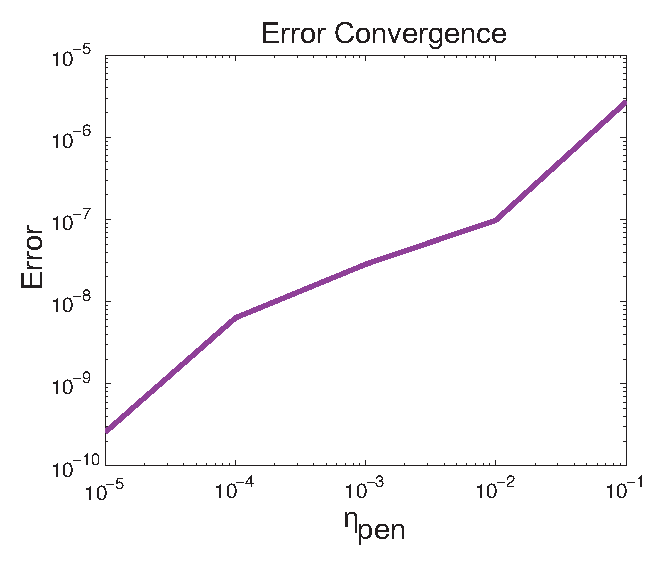
\includegraphics[width=3 in]{Images/errorconverge_noslip.eps}
  \caption[Error convergence for no slip conditions]{A plot of error convergence for decreasing penalization parameter for no slip condtions..}\label{f:errorconverge_noslip}
\end{figure}
\end{center}

Comparison of the solution profiles demonstrates accurate representation of no slip conditions using this method.  However, for the large scale ocean modeling of interest, no slip boundary conditions are not necessary or realistic. To avoid resolving the boundary layer associated with no slip conditions, it was necessary to extend this methodology to slip conditions, $\frac{\partial u}{\partial z}=\kappa u$.  The idea is very similar to the no slip case, although, some numerical complications arose that made its implementation slightly more complicated.  Figure \ref{f:fluxdiagram} shows a schematic of the equations to be solved in each region for slip conditions to be satisfied.

\begin{center}
\begin{figure}[htp]
\centering
  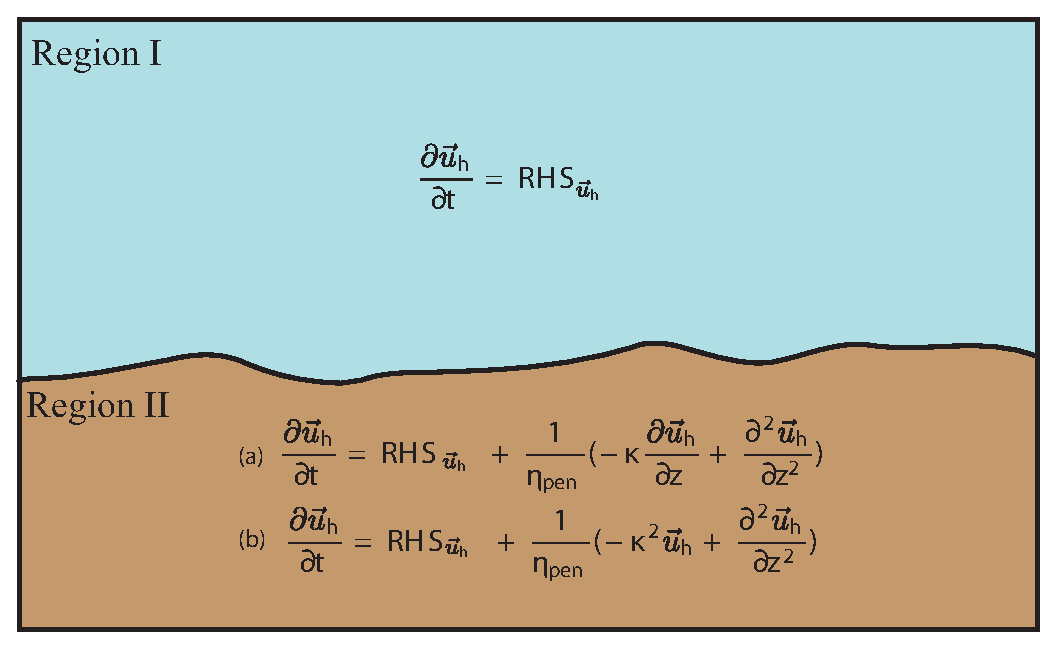
\includegraphics[width=4 in]{Images/fluxdiagram.eps}
  \caption[Diagram of two formulations of extension of Brinkman to slip conditions]{Diagram of how Brinkman penalization can be extended to slip conditions with the equations needed to be solved in each region.}\label{f:fluxdiagram}
\end{figure}
\end{center}

Two different volume penalization methods were developed and tested.  The full set of penalized governing equations are, 
%
\begin{equation*}\label{e:seasurfaceheightpen2}
\frac{\partial \eta}{\partial t} + ({\bf u}_{h}|_{z=z_{max}}) \cdot \nabla_{h} \eta = (w|_{z=z_{max}})
\end{equation*}
(a)
\begin{equation*} \label{e:momentumpen2}
\frac{\partial {\bf u}_{h}}{\partial t} + {\bf u} \cdot \nabla {\bf u}_{h} + \frac{1}{Ro} f \hat{\bf k} \times {\bf u}_{h}= -\nabla_{h} P + \frac{1}{Re} \nabla ^{2} {\bf u}_{h} +   \frac{\chi}{\eta_{pen}} \left(-\kappa \frac{\partial {\bf u}_{h}}{\partial z} + \frac{\partial^{2} {\bf u_{h}}}{\partial z^{2}} \right)
\end{equation*}
(b)
\begin{equation*} \label{e:momentumpen2}
\frac{\partial {\bf u}_{h}}{\partial t} + {\bf u} \cdot \nabla {\bf u}_{h} + \frac{1}{Ro} f \hat{\bf k} \times {\bf u}_{h}= -\nabla_{h} P + \frac{1}{Re} \nabla ^{2} {\bf u}_{h} +  \frac{\chi}{\eta_{pen}} \left(-\kappa^{2} {\bf u}_{h} + \frac{\partial^{2} {\bf u_{h}}}{\partial z^{2}} \right)
\end{equation*}

\begin{equation*}\label{e:continuitypen2}
 \frac{\partial w}{\partial z} = - \nabla_{h}{\bf u}_{h}, (w|_{z=z_{bottom}({\bf x_{h}})})=0
\end{equation*}

\begin{equation*}\label{e:hydrostaticpressurepen2}
\frac{\partial P}{\partial z} = -\frac{1}{Fr^{2}}, P|_{z=z_{max}} = \frac{\eta}{Fr^{2}}
\end{equation*}
where,

 \begin{equation*}\label{e:chi}
   \chi=\begin{cases}
   1&\text{if } x \in O_{i}\\
   0&\text{otherwise} \end{cases}
 \end{equation*}
 %
and (a) and (b) are the two different volume penalization options.  It was found that both methods converged to the numerical results that do not use penalization equally as well for a flat boundary interface.  Figure \ref{f:error_diffmeth} shows the error of the two methods and shows the comparison of the velocity profiles in a horizontal slice of all three methods.  These results are shown for $\kappa=10$, which causes a steeper slope in the velocity as it approaches the bottom boundary and allows for better visual comparison.

\begin{center}
\begin{figure}[htp]
\centering
  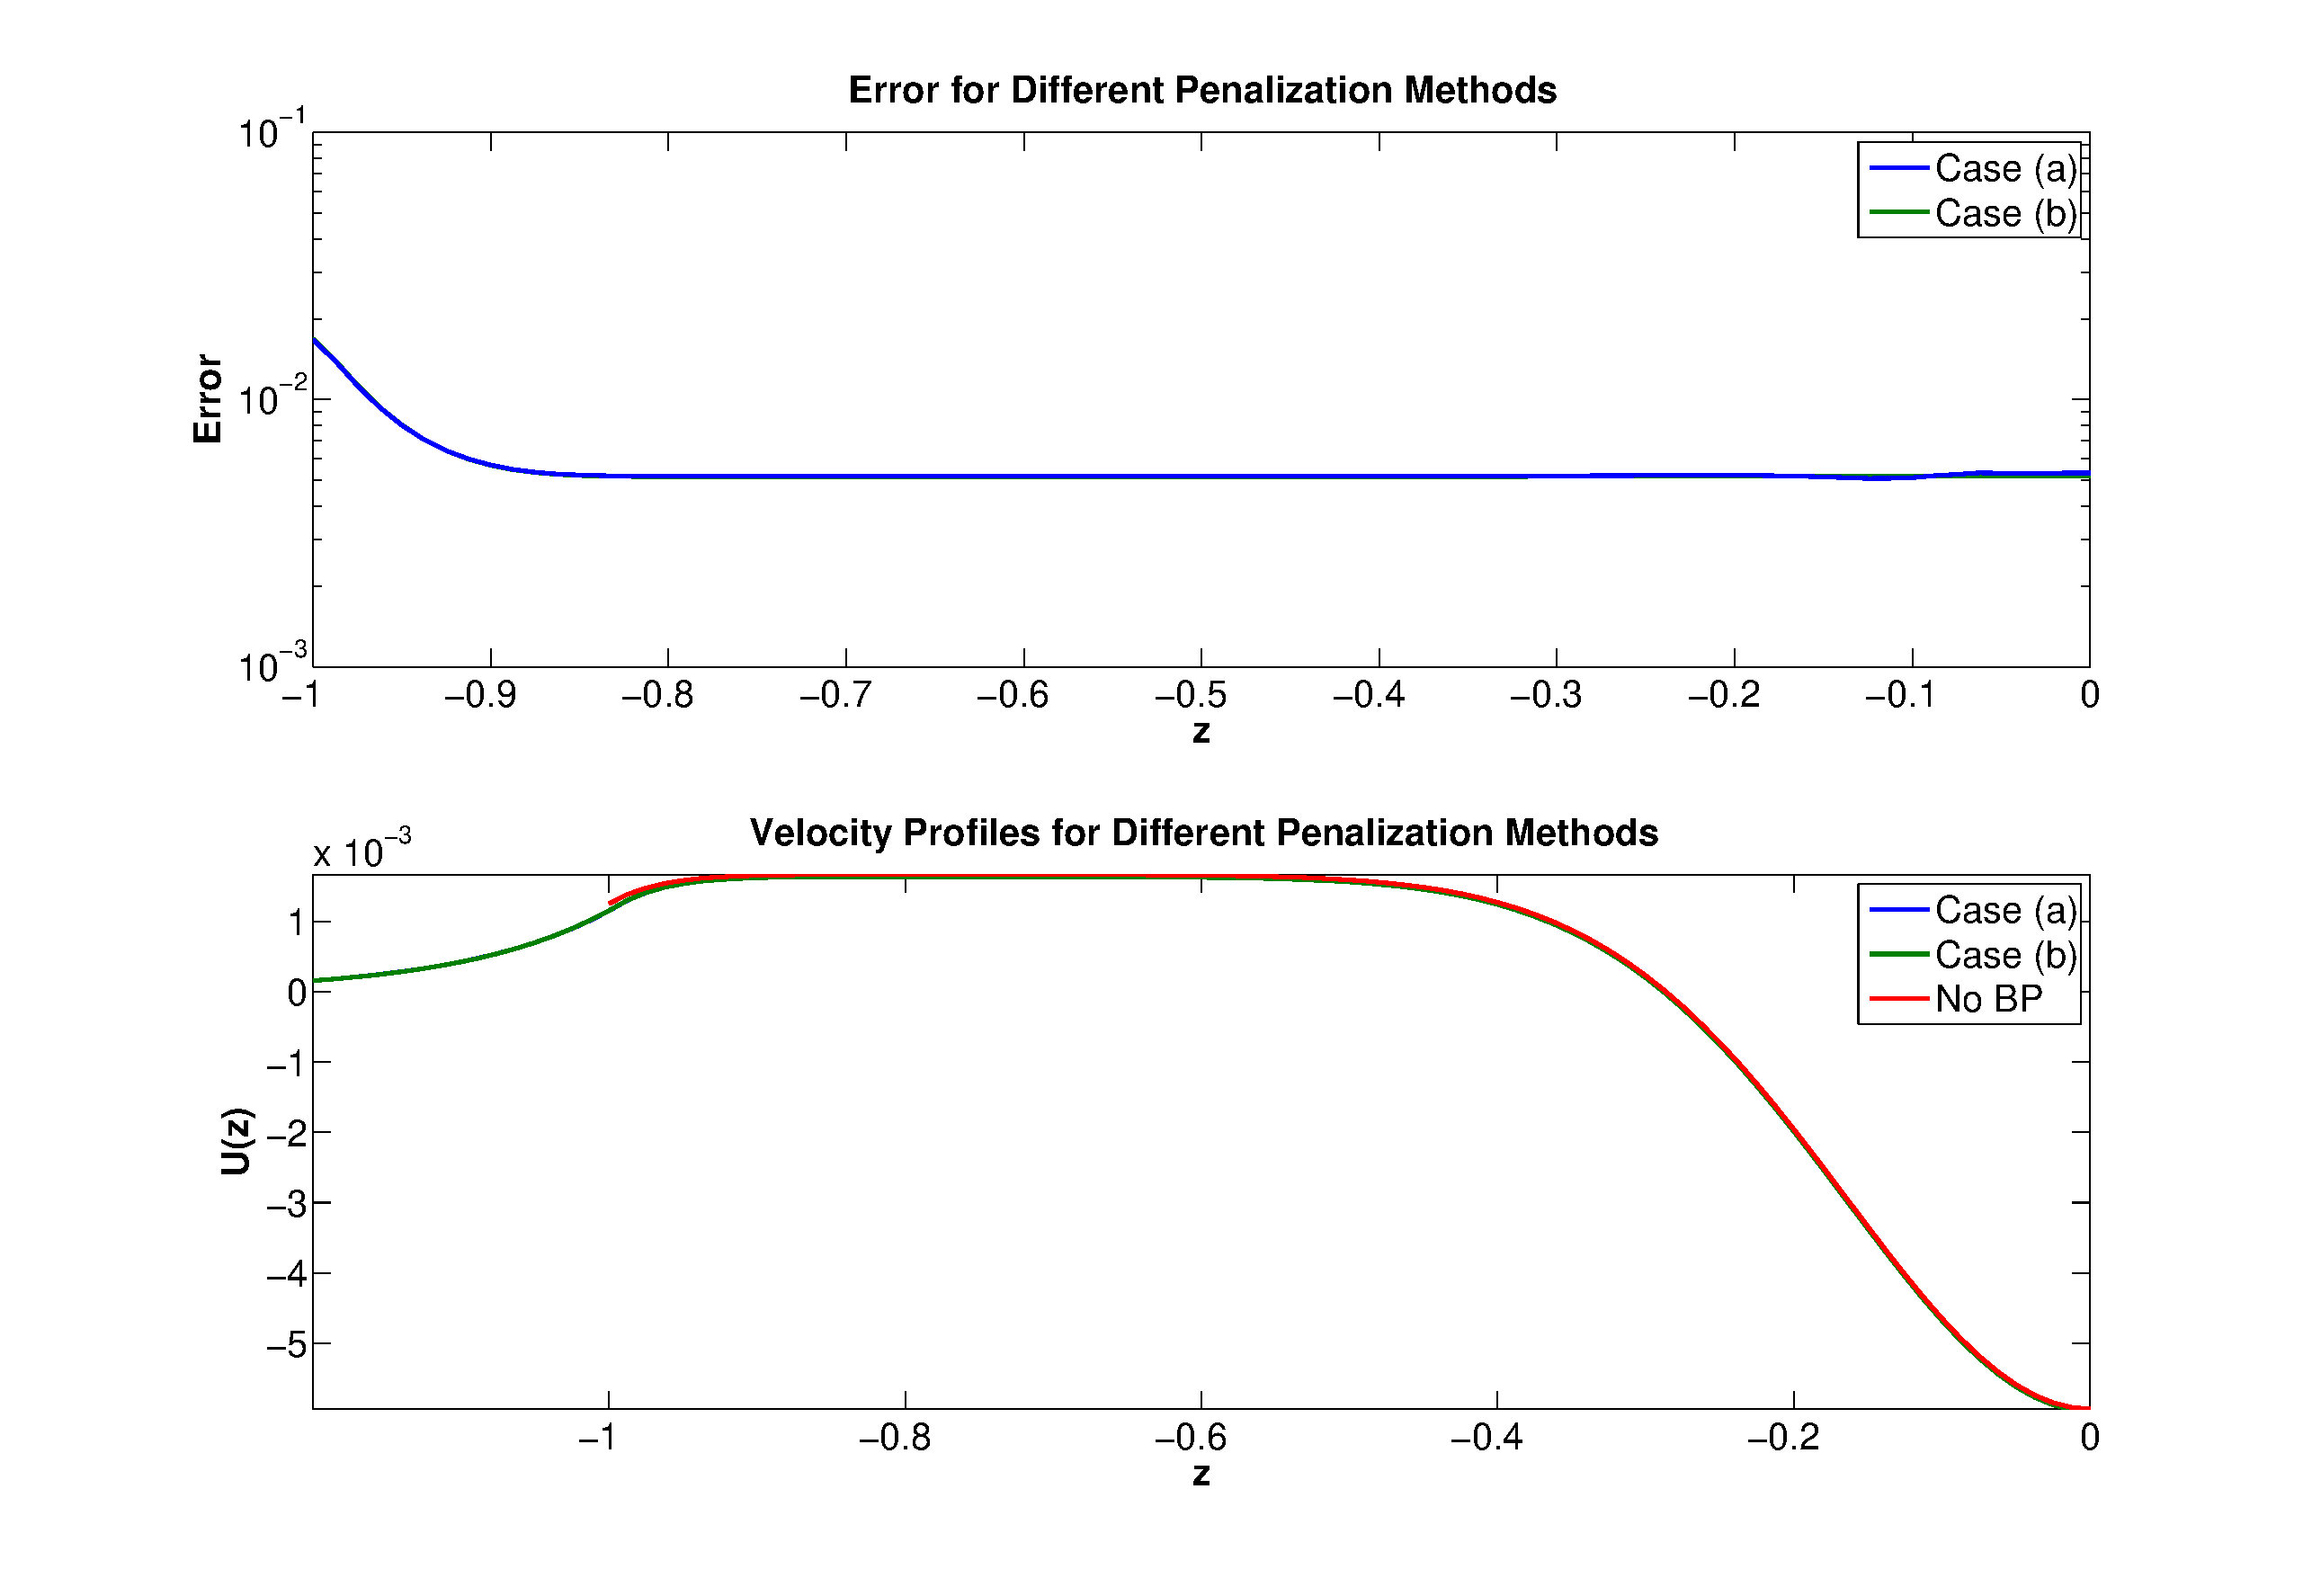
\includegraphics[width=5 in]{Images/error_diffmeth.eps}
  \caption[Comparison of two Brinkman methods for slip conditions]{Top: the error of the two penalization methods (a) and (b) computed against numerical results from non-penalized implementation of slip boundary conditions. Bottom: the velocity profiles of all three methods (two penalization method and non-penalized approach for a slice at $x=0.5$.}\label{f:error_diffmeth}
\end{figure}
\end{center}


It was also found the value of $\kappa$ does make for a drastically different velocity profile.  Figures \ref{f:slip} and \ref{f:slipk10} show plots of velocity and the adaptive grid for both $\kappa=1$ and $\kappa=10$.  Additionally, as a result of the steeper slope in a higher $\kappa$ value, there is a finer resolution near the penalization zone.  

\begin{center}
\begin{figure}[htp]
\centering
  \includegraphics[width=6 in]{Images/pe_bp_slip_k1.eps}
  \caption[Slip conditions, $\kappa=1$, with and without penalization]{Demonstration of slip boundary conditions with and without Brinkman penalization for $\kappa=1$.}\label{f:slip}
\end{figure}
\end{center}

\begin{center}
\begin{figure}[htp]
\centering
  \includegraphics[width=6 in]{Images/pe_bp_slip_k10.eps}
  \caption[Slip conditions, $\kappa=10$, with and without penalization]{Demonstration of slip boundary conditions with and without Brinkman penalization for $\kappa=10$.}\label{f:slipk10}
\end{figure}
\end{center}

Figure \ref{f:error_diffmeth} shows that the slopes of velocity along the vertical direction in the penalized case are not exactly equivalent to the non-penalized case.  Further investigation has begun to see if this solution will converge to the non-penalized solution as the penalization parameter, $\eta_{pen}$ is decreased.  A preliminary study has been done and is shown in Figure \ref{f:errorconverge_slip}.  Although, the convergence is not as good as the no slip Brinkman penalization, it still may be more than sufficient.  

\begin{center}
\begin{figure}[htp]
\centering
  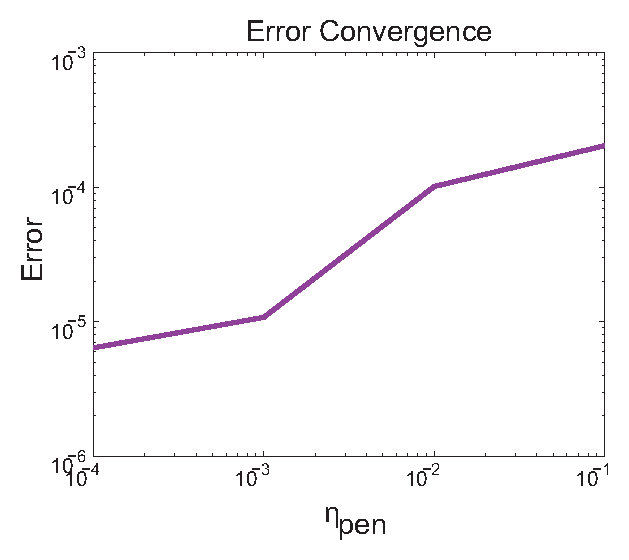
\includegraphics[width=3 in]{Images/errorconverge_slip.eps}
  \caption[Error convergence for slip conditions]{A plot of error convergence for decreasing penalization parameter for slip condtions.}\label{f:errorconverge_slip}
\end{figure}
\end{center}
